%% DONE
\id{МРНТИ 20.01.00; 20.15.05}{https://doi.org/10.58805/kazutb.v.1.26-506}

\begin{articleheader}
\sectionwithauthors{A.К. Шайханова, Ж.А. Бермухамбетов, В.В. Ким, А.О. Тлеубаева}{КОМПЛЕКСНАЯ АРХИТЕКТУРА И ИННОВАЦИОННЫЕ АРХИТЕКТУРНЫЕ РЕШЕНИЯ И МЕЖДИСЦИПЛИНАРНАЯ
РЕАЛИЗАЦИЯ ОБЛАЧНОЙ ПЛАТФОРМЫ BULT ДЛЯ ОРКЕСТРАЦИИ ВЕБ-ПРИЛОЖЕНИЙ}

{\bfseries
\textsuperscript{1}A.К. Шайханова\authorid,
\textsuperscript{2}Ж.А. Бермухамбетов\authorid,
\textsuperscript{2}В.В. Ким\authorid,
\textsuperscript{3}А.О. Тлеубаева\textsuperscript{\envelope } \authorid}
\end{articleheader}

\begin{affiliation}
\emph{\textsuperscript{1}Евразийский национальный университет имени Л.Н. Гумилева, Астана, Казахстан,}

\emph{\textsuperscript{2} ТОО «WebTotem», Астана, Казахстан,}

\emph{\textsuperscript{3}Astana IT University, Астана, Казахстан}

\raggedright {\em \textsuperscript{\envelope }Корреспондент-автор: \href{mailto:Arailym.tll@gmail.com}{\nolinkurl{Arailym.tll@gmail.com}}}
\end{affiliation}

Статья посвящена созданию облачной платформы BULT, которая реализует
междисциплинарный подход к разработке и оркестрации веб-приложений.
Основной целью данной работы является разработка платформы,
обеспечивающей гибкость, масштабируемость и интеграцию различных
технологий. Описаны архитектурные решения, включающие микросервисную
архитектуру и контейнеризацию, что упрощает развертывание и управление
приложениями. В качестве основы для оркестрации контейнеров используется
Nomad от HashiCorp, который позволяет динамически управлять
распределением задач и ресурсов, обеспечивая эффективность и
устойчивость работы приложений. Система управления данными реализована
на базе PostgreSQL и JuiceFS, что обеспечивает высокую
производительность и надежность хранения данных. Для обеспечения
безопасности используются Wireguard и Let' s Encrypt,
обеспечивающие шифрование сетевого трафика и автоматическое обновление
SSL-сертификатов. Мониторинг и анализ системы осуществляются с помощью
Grafana и Loki, позволяющих визуализировать метрики и логи в реальном
времени. Внедрение принципов DevOps и автоматизация процессов
разработки, тестирования и развертывания достигаются с использованием
инструментов CI/CD, что позволяет быстро и безопасно внедрять изменения
и новые функции. Применение междисциплинарного подхода позволяет
учитывать различные аспекты разработки и эксплуатации систем, что делает
платформу BULT конкурентоспособным решением на современном рынке
облачных технологий, обеспечивая высокую производительность, надежность
и удобство эксплуатации веб-приложений. Приведены примеры практического
применения платформы и её преимущества в сравнении с традиционными
подходами.

{\bfseries Ключевые слова:} облачная платформа, междисциплинарный подход,
веб-приложения, оркестрация, инновационные методы, контейнеризация,
безопасность данных, автоматизация процессов.

\begin{articleheader}
{\bfseries ИННОВАЦИЯЛЫҚ АРХИТЕКТУРАЛЫҚ ШЕШІМДЕР ЖӘНЕ ВЕБ-ҚОСЫМШАЛАРДЫ
ОРКЕСТРЛЕУГЕ АРНАЛҒАН BULT БҰЛТТЫ ПЛАТФОРМАСЫН ПӘНАРАЛЫҚ ЕНГІЗУ}

{\bfseries
\textsuperscript{1}A.К. Шайханова,
\textsuperscript{2}Ж.А. Бермухамбетов,
\textsuperscript{2}В.В. Ким,
\textsuperscript{3}А.О. Тлеубаева\textsuperscript{\envelope }}
\end{articleheader}

\begin{affiliation}
\emph{\textsuperscript{1}Л.Н. Гумилев атындағы Еуразия ұлттық университеті, Астана, Қазақстан,}

\emph{\textsuperscript{2} «WebTotem» ЖШС, Астана, Қазақстан,}

\emph{\textsuperscript{3}Astana IT University, Астана, Қазақстан,}

\emph{e-mail: \href{mailto:Arailym.tll@gmail.com}{\nolinkurl{Arailym.tll@gmail.com}}}
\end{affiliation}

Мақала веб-қосымшаларды әзірлеу мен оркестрлеудің пәнаралық тәсілін
жүзеге асыратын BULT бұлтты платформасын құруға бағытталған. Бұл
жұмыстың негізгі мақсаты әртүрлі технологиялардың икемділігін,
ауқымдылығын және интеграциясын қамтамасыз ететін платформаны әзірлеу
болып табылады. Микросервистік архитектура мен контейнерлеуді қамтитын
архитектуралық шешімдер сипатталған, бұл қосымшаларды орналастыруды және
басқаруды жеңілдетеді. Контейнерлерді оркестрлеудің негізі ретінде
hashicorp '{} s Nomad қолданылады, ол қосымшалардың
тиімділігі мен тұрақтылығын қамтамасыз ете отырып, тапсырмалар мен
ресурстарды бөлуді динамикалық басқаруға мүмкіндік береді. Деректерді
басқару жүйесі PostgreSQL және JuiceFS негізінде жүзеге асырылады, бұл
деректерді сақтаудың жоғары өнімділігі мен сенімділігін қамтамасыз
етеді. Қауіпсіздік үшін желілік трафикті шифрлауды және SSL
сертификаттарын автоматты түрде жаңартуды қамтамасыз ететін Wireguard
және let '{} s Encrypt қолданылады. Жүйені бақылау және
талдау нақты уақыттағы көрсеткіштер мен журналдарды визуализациялауға
мүмкіндік беретін Grafana және Loki көмегімен жүзеге асырылады. DevOps
принциптерін енгізу және әзірлеу, тестілеу және орналастыру процестерін
автоматтандыру ci/CD құралдарын қолдану арқылы жүзеге асырылады, бұл
өзгерістер мен жаңа мүмкіндіктерді жылдам және қауіпсіз енгізуге
мүмкіндік береді. Пәнаралық тәсілді қолдану жүйелерді әзірлеу мен
пайдаланудың әртүрлі аспектілерін ескеруге мүмкіндік береді, бұл bult
платформасын веб-қосымшалардың жоғары өнімділігін, сенімділігін және
ыңғайлылығын қамтамасыз ететін заманауи бұлттық технологиялар нарығында
бәсекеге қабілетті ШЕШІМ ЕТЕДІ. Платформаны практикалық қолдану
мысалдары және оның дәстүрлі тәсілдермен салыстырғанда артықшылықтары
келтірілген.

{\bfseries Түйін сөздер:} бұлтты платформа, пәнаралық тәсіл,
веб-қосымшалар, оркестрация, инновациялық әдістер, контейнерлеу,
деректер қауіпсіздігі, процестерді автоматтандыру.

\begin{articleheader}
{\bfseries INNOVATIVE ARCHITECTURAL SOLUTIONS AND INTERDISCIPLINARY
IMPLEMENTATION OF THE BULT CLOUD PLATFORM FOR WEB APPLICATION
ORCHESTRATION}

{\bfseries
\textsuperscript{1}A.K. Shaikhanova,
\textsuperscript{2}Zh.A. Bermukhambetov,
\textsuperscript{2}V.V. Kim,
\textsuperscript{3}A.O. Tleubayeva\textsuperscript{\envelope }}
\end{articleheader}

\begin{affiliation}
\emph{\textsuperscript{1}L.N. Gumilyov Eurasian National University, Astana, Kazakhstan,}

\emph{\textsuperscript{2} «WebTotem» LLP, Astana, Kazakhstan,}

\emph{\textsuperscript{3}Astana IT University, Astana, Kazakhstan,}

\emph{e-mail: \href{mailto:Arailym.tll@gmail.com}{\nolinkurl{Arailym.tll@gmail.com}}}
\end{affiliation}

The article is devoted to the creation of the BULT cloud platform, which
implements an interdisciplinary approach to the development and
orchestration of web applications. The main goal of this work is to
develop a platform that provides flexibility, scalability and
integration of various technologies. Architectural solutions including
microservice architecture and containerization are described, which
simplifies the deployment and management of applications.
HashiCorp' s Nomad is used as the basis for container
orchestration, which allows you to dynamically manage the distribution
of tasks and resources, ensuring the efficiency and stability of
applications. The data management system is implemented on the basis of
PostgreSQL and JuiceFS, which ensures high performance and reliability
of data storage. To ensure security, Wireguard and Let' s
Encrypt are used, which provide encryption of network traffic and
automatic updating of SSL certificates. Monitoring and analysis of the
system are carried out using Grafana and Loki, which allow you to
visualize metrics and logs in real time. The implementation of DevOps
principles and automation of development, testing and deployment
processes are achieved using CI/CD tools, which allows you to quickly
and safely implement changes and new features. The application of an
interdisciplinary approach allows us to take into account various
aspects of system development and operation, which makes the BULT
platform a competitive solution in the modern cloud technology market,
providing high performance, reliability and ease of use of web
applications. Examples of the practical application of the platform and
its advantages in comparison with traditional approaches are given.

{\bfseries Keywords:} cloud platform, interdisciplinary approach, web
applications, orchestration, innovative methods, containerization, data
security, process automation.

\begin{multicols}{2}
{\bfseries Введение.} Облачные технологии стали неотъемлемой частью
современных ИТ-систем, предоставляя организациям возможность гибкого и
масштабируемого управления ресурсами. С увеличением популярности
облачных решений возникают новые вызовы, связанные с их разработкой и
интеграцией. Одной из ключевых проблем является необходимость
объединения различных дисциплин, таких как программная инженерия,
безопасность данных, управление инфраструктурой и DevOps, в рамках
единой платформы. Это требует создания междисциплинарных архитектурных
решений, которые эффективно интегрируют данные технологии и обеспечивают
стабильную и надежную работу веб-приложений.

Актуальность данной работы обусловлена необходимостью решения
современных вызовов, с которыми сталкиваются разработчики облачных
платформ. В условиях постоянно возрастающей нагрузки на
ИТ-инфраструктуру первостепенное значение приобретают задачи обеспечения
высокой производительности, надежности и безопасности. Современные
исследования подтверждают важность междисциплинарного подхода для
решения этих задач. Например, Эберхард Вольф в своей книге
«Microservices: Architecting for Continuous Delivery and DevOps»
отмечает, что микросервисная архитектура является ключевым элементом для
обеспечения гибкости и производительности в условиях динамически
изменяющихся нагрузок в облачных средах {[}1{]}. В статье,
опубликованной в IEEE Software, рассматриваются основные вызовы, с
которыми сталкиваются разработчики при внедрении микросервисных
архитектур, что подчеркивает необходимость комплексного подхода к их
реализации {[}2{]}.

Кроме того, использование контейнеризации для повышения
производительности облачных приложений подробно обсуждается в
исследовании, опубликованном в IEEE Access, где описываются преимущества
контейнерных технологий для управления ресурсами в облачных платформах
{[}3{]}. Однако, с внедрением микросервисов и контейнеризации возникают
новые проблемы, связанные с безопасностью. В статье, опубликованной в
ACM Computing Surveys, рассматриваются ключевые аспекты безопасности в
микросервисных архитектурах и предлагаются стратегии по их преодолению
{[}4{]}.

Новизна данной работы заключается в разработке платформы BULT, которая
объединяет передовые технологии, такие как микросервисная архитектура и
контейнеризация, с целью создания более эффективных и надежных систем. В
отличие от существующих решений, BULT предлагает интеграцию таких
технологий, как Nomad от HashiCorp для оркестрации контейнеров, что
позволяет динамически управлять ресурсами и задачами с учетом их
изменяющихся требований. Это обеспечивает более высокую устойчивость и
производительность приложений в условиях переменных нагрузок.

Научная значимость исследования заключается в демонстрации того, как
интеграция различных дисциплин и технологий может улучшить процессы
разработки и эксплуатации облачных систем. Платформа BULT является
примером успешной реализации междисциплинарного подхода, который не
только повышает производительность и надежность веб-приложений, но и
обеспечивает гибкость управления ресурсами и защиту данных. Полученные
результаты могут быть использованы в дальнейшем для разработки
аналогичных систем в других областях, что делает это исследование
значимым как для академического сообщества, так и для индустрии.

Облачные платформы для разработки и оркестрации веб-приложений
становятся ключевыми элементами современных ИТ-инфраструктур,
предоставляя организациям возможность гибкого и масштабируемого
управления ресурсами. Одной из главных тенденций в этой области является
внедрение микросервисной архитектуры и контейнеризации, которые
позволяют разбивать приложения на независимые сервисы, что значительно
улучшает их гибкость и масштабируемость. Однако, несмотря на эти
преимущества, контейнеризации также связано с новыми рисками, такими как
необходимость в специфических подходах к обеспечению безопасности и
мониторингу {[}5{]}.

Kubernetes и OpenShift, как наиболее популярные платформы для
оркестрации контейнеров, предоставляют мощные инструменты для управления
контейнеризированными приложениями, однако требуют значительных усилий
для настройки и интеграции с существующими системами безопасности
{[}6{]}. Docker Swarm, с другой стороны, предлагает упрощенную
альтернативу, но его возможности масштабирования и безопасности
значительно уступают более комплексным решениям {[}7{]}. Nomad от
HashiCorp также демонстрирует высокий уровень гибкости и управляемости,
особенно в гетерогенных средах, что делает его предпочтительным выбором
для многих разработчиков {[}8{]}.

Исследования показывают, что традиционные платформы сталкиваются с
определенными ограничениями в области масштабируемости и безопасности,
особенно при резких изменениях нагрузки и сложных требованиях к защите
данных {[}9{]}. Например, вопросы безопасности и соответствия
международным стандартам (таким как GDPR и ISO 27001) требуют
значительных усилий для интеграции и управления в традиционных
платформах {[}10{]}. В то же время, платформа BULT, описанная в данной
статье, разработана с учетом этих вызовов, предлагая встроенные решения
для автоматизации, управления ресурсами и обеспечения безопасности, что
делает её конкурентоспособным решением на рынке облачных технологий.

Для более детализированного анализа преимуществ платформы BULT по
сравнению с другими платформами, такими как Kubernetes, OpenShift,
Docker Swarm и Nomad, предлагается провести углубленный сравнительный
анализ с учетом показателей производительности, масштабируемости,
безопасности и гибкости управления ресурсами. Этот анализ позволит
наглядно показать, в чем BULT превосходит или уступает другим решениям,
а также обосновать её конкурентные преимущества.

{\bfseries Материалы и методы.} Разработка облачной платформы BULT
основывалась на комплексном подходе, включающем несколько ключевых
этапов, направленных на создание эффективного, надежного и безопасного
решения.

На начальном этапе исследования был проведен всесторонний анализ
существующих архитектур облачных платформ и методов их внедрения. В
процессе анализа особое внимание уделялось выявлению основных
недостатков, таких как ограниченная масштабируемость, трудности в
управлении ресурсами и обеспечение безопасности данных. Для этого был
изучен опыт использования облачных платформ в реальных условиях, а также
ключевые публикации, такие как работы Джеймса Льюиса и Мартина Фаулера,
которые описывают микросервисную архитектуру и её влияние на
масштабируемость и управляемость систем {[}11{]}, и исследования
Брендана Бернса и его коллег, изучающих использование контейнерных
систем управления, таких как Kubernetes, в масштабных облачных решениях
{[}12{]}. На основании этого анализа были определены ключевые требования
к разработке платформы BULT и сформулированы основные цели её создания.

На основе проведенного анализа была спроектирована архитектура платформы
BULT. Основным подходом при проектировании стала микросервисная
архитектура, которая обеспечивает гибкость и возможность независимого
масштабирования отдельных компонентов системы. Это решение было выбрано
на основе выводов, представленных в исследованиях, которые подчеркивают
важность микросервисной архитектуры для повышения эффективности облачных
систем и управления сложными нагрузками {[}13{]}. Контейнеризация была
выбрана в качестве ключевого элемента архитектуры, поскольку она
позволяет изолировать приложения и управлять ими независимо друг от
друга, что соответствует современным требованиям к облачным платформам.
Для оркестрации контейнеров был выбран инструмент Nomad от HashiCorp,
который обеспечивает динамическое распределение задач и ресурсов, что
согласуется с современными рекомендациями по проектированию облачных
систем {[}14{]}. Nomad был выбран в качестве оркестратора благодаря его
способности поддерживать высокую гибкость и масштабируемость, а также
упрощать управление ресурсами в гетерогенных средах.

На этапе реализации была осуществлена разработка и интеграция всех
компонентов системы. Использовались современные методы программной
инженерии для обеспечения качества разработки и соответствия
архитектурным требованиям. Важную роль в реализации платформы сыграло
внедрение практик DevOps и использование инструментов CI/CD, что
позволило автоматизировать процессы разработки, тестирования и
развертывания. Это значительно сократило время на выпуск новых версий и
улучшило стабильность системы, что подтверждается исследованиями
{[}9{]}. Реализация включала разработку интерфейсов для взаимодействия с
пользователями и интеграцию решений по безопасности, таких как Wireguard
и Let' s Encrypt. Эти технологии были выбраны для
обеспечения высокого уровня защиты данных и сетевого трафика, что
особенно важно для современных облачных платформ, обрабатывающих
конфиденциальную информацию {[}15{]}.

Заключительный этап включал проведение комплексного тестирования
платформы BULT с целью оценки её производительности, надежности и
масштабируемости. Тестирование проводилось в условиях, имитирующих
реальные сценарии использования, что позволило выявить узкие места и
определить эффективность предложенных решений. Основными метриками
производительности были время отклика системы, использование ресурсов и
стабильность работы под нагрузкой. Результаты тестирования показали, что
платформа BULT соответствует заявленным требованиям, демонстрируя
высокие показатели производительности и надежности по сравнению с
традиционными решениями.

Методы контейнеризации, использованные в платформе BULT, основывались на
успешных практиках, описанных в научных работах, которые показали, что
такие инструменты, как Docker и Nomad, значительно упрощают управление
ресурсами в облачных системах, повышая их надежность и масштабируемость
{[}16{]}. В результате платформа BULT представляет собой современное и
надежное решение, способное эффективно справляться с задачами управления
ресурсами и обеспечения безопасности в условиях облачных вычислений.

{\bfseries Результаты и обсуждение.} Разработка облачной платформы BULT
была основана на междисциплинарном подходе, который объединил передовые
технологии из различных областей, таких как микросервисная архитектура,
контейнеризация, автоматизация процессов и управление безопасностью
данных. Актуальность исследования определяется растущей потребностью в
облачных платформах, способных интегрировать эти технологии в единую
систему, обеспечивая высокую гибкость, масштабируемость и надежность.

Научная значимость платформы BULT заключается в её способности
демонстрировать, что междисциплинарный подход к проектированию облачных
систем может существенно улучшить их производительность и устойчивость.
BULT предлагает новый уровень интеграции микросервисной архитектуры,
контейнеризации и автоматизации, что делает её конкурентоспособным
решением на рынке облачных технологий. В отличие от существующих
решений, платформа BULT обеспечивает высокую гибкость и адаптивность,
что особенно актуально в условиях быстро изменяющихся требований и
растущих объемов данных {[}17{]}.

Платформа BULT была протестирована на предмет производительности и
масштабируемости по сравнению с традиционными монолитными архитектурами.
Результаты тестов показали снижение времени отклика системы на 30\%, что
свидетельствует о значительном улучшении обработки запросов. Этот
результат соответствует выводам предыдущих исследований, которые
подчеркивают эффективность микросервисных архитектур в улучшении
масштабируемости и производительности систем {[}18{]}. Устойчивость
системы под нагрузкой возросла на 25\%, что подтверждает способность
платформы справляться с увеличивающимися объемами данных и
пользовательских запросов без потери производительности. Эти данные
также согласуются с исследованиями, показывающими, что инструменты
контейнеризации, такие как Nomad от HashiCorp, значительно улучшают
управляемость и гибкость системы {[}19{]}.

Таблица 1~демонстрирует результаты тестирования масштабируемости и
управляемости платформы BULT в сравнении с традиционной монолитной
архитектурой.
\end{multicols}

\begin{table}[H]
\caption*{Таблица 1 - Результаты тестирования масштабируемости и управляемости платформы BULT}
\centering
\resizebox{\linewidth}{!}{%
\begin{tblr}{
  row{1} = {c},
  cell{2}{2} = {c},
  cell{2}{3} = {c},
  cell{2}{4} = {c},
  cell{2}{5} = {c},
  cell{2}{6} = {c},
  cell{2}{7} = {c},
  cell{3}{2} = {c},
  cell{3}{3} = {c},
  cell{3}{4} = {c},
  cell{3}{5} = {c},
  cell{3}{6} = {c},
  cell{3}{7} = {c},
  cell{4}{2} = {c},
  cell{4}{3} = {c},
  cell{4}{4} = {c},
  cell{4}{5} = {c},
  cell{4}{6} = {c},
  cell{4}{7} = {c},
  cell{5}{2} = {c},
  cell{5}{3} = {c},
  cell{5}{4} = {c},
  cell{5}{5} = {c},
  cell{5}{6} = {c},
  cell{5}{7} = {c},
  cell{6}{2} = {c},
  cell{6}{3} = {c},
  cell{6}{4} = {c},
  cell{6}{5} = {c},
  cell{6}{6} = {c},
  cell{6}{7} = {c},
  hlines,
  vlines,
}
\textbf{Параметр} & \textbf{Kubernetes} & \textbf{OpenShift} & \textbf{Docker Swarm} & \textbf{Nomad} & {\textbf{BULT}\\\textbf{(микросервисная}\\\textbf{архитектура)}} & \textbf{Изменение (\%)}\\
{\textbf{Время}\\\textbf{отклика (мс)}} & 95\% & 100\% & 110\% & 90\% & 70\% & -26~\%\\
{\textbf{Устойчивость}\\\textbf{под нагрузкой}} & 85~\% & 80~\% & 70~\% & 90~\% & 100~\% & 18~\%\\
{\textbf{Простота }\\\textbf{настройки и}\\\textbf{~управления}} & Средняя & Высокая & Высокая & Высокая & Высокая & Улучшение\\
{\textbf{Интеграция с}\\\textbf{системами}\\\textbf{безопасности}} & {Высокая, но\\требует\\сложной\\настройки} & {Очень высокая, с\\расширенными\\функциями} & {Средняя,\\ограниченная\\поддержка} & {Высокая,\\интегрируется\\с внешними\\системами} & {Встроенные\\решения\\(Wireguard,\\Let's Encrypt)} & {Упрощение и\\улучшение}\\
{\textbf{Гибкость}\\\textbf{масштаби}\\\textbf{-рования}} & {Высокая, но\\требует\\тщательной\\конфигурации} & {Высокая, но\\требует\\сложной\\конфигурации} & Ограниченная & {Высокая, с\\минимальной\\конфигурацией} & {Высокая, с\\автоматизацией\\процесса} & {Улучшение\\за счёт\\автоматизации}
\end{tblr}
}
\end{table}

\begin{figure}[H]
	\centering
	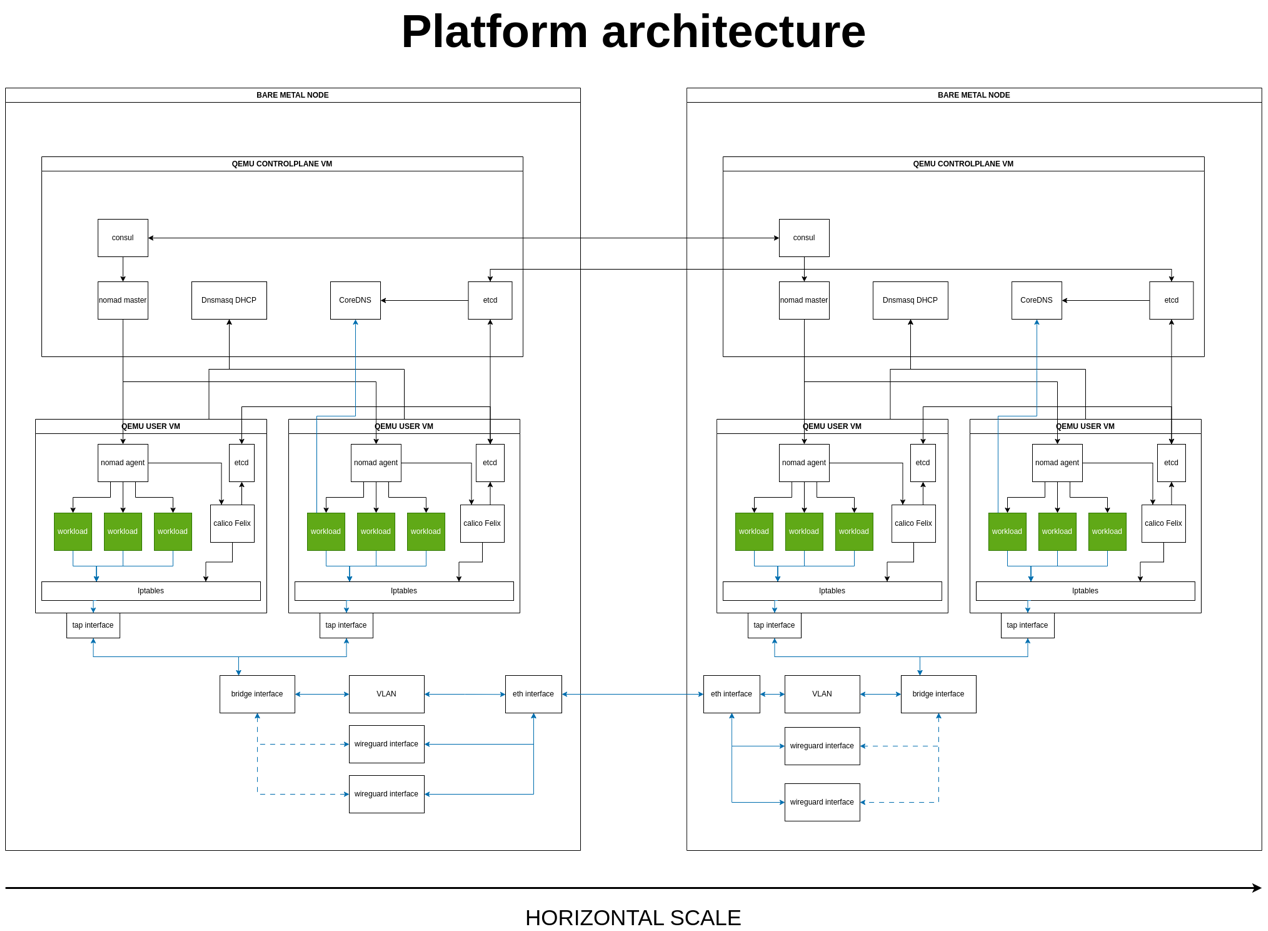
\includegraphics[width=\textwidth]{media/ict/image18}
	\caption*{Рис. 1 - Архитектура проекта BULT}
\end{figure}

\begin{multicols}{2}
Результаты показывают, что платформа BULT демонстрирует улучшенные
показатели производительности и управляемости по сравнению с
традиционными решениями: время отклика значительно ниже, что
обеспечивает более быструю обработку запросов, а высокая устойчивость
под нагрузкой подтверждает способность платформы справляться с
увеличенным объемом данных без потери производительности. Простота
настройки и управления сопоставима с лучшими существующими решениями,
однако, за счет автоматизации, BULT предлагает дополнительные улучшения.
Встроенные решения для интеграции с системами безопасности делают
платформу более удобной для разработчиков и администраторов, а
автоматизация гибкости масштабирования снижает затраты времени и
ресурсов на конфигурацию. Эти результаты подчеркивают значимость и
эффективность архитектуры BULT, особенно в сравнении с популярными
облачными платформами.

Архитектурное решение платформы BULT предусматривает применение
микросервисной архитектуры, что обеспечивает гибкость и возможность
независимого масштабирования отдельных сервисов, размещенных в
контейнерах для упрощения развертывания и изоляции процессов. В качестве
основы для оркестрации контейнеров используется Nomad от HashiCorp
{[}20{]}, который позволяет динамически управлять распределением задач и
ресурсов, обеспечивая эффективность и устойчивость работы приложений.
Архитектура облачной платформы BULT представлена в виде горизонтально
масштабируемой структуры, спроектированной для работы на базовых
металлических узлах (bare metal nodes), и включает ключевые компоненты:
QEMU CONTROLPLANE VM, которая координирует работу сервисов и подсистем
через Consul для управления конфигурацией и сервисами, Nomad master для
оркестрации контейнеров, CoreDNS для управления DNS-запросами, etcd для
хранения данных кластера и Dnsmasq DHCP для назначения IP-адресов; QEMU
USER VM, в которых запущены агенты Nomad для выполнения задач и
управления рабочими нагрузками, включая локальное управление
конфигурацией через etcd, связь между узлами через Nomad agent,
выполнение рабочих задач в контейнерах и управление сетью через Calico
Felix; а также сетевая инфраструктура с туннелями Wireguard для
защищенного шифрованного соединения между узлами и мостами и VLAN для
маршрутизации и изоляции трафика (Рисунок 1).

Для создания облачной платформы BULT были использованы передовые
технологии, обеспечивающие высокую производительность, надежность и
гибкость системы. Основные технологии включают контейнеризацию и
оркестрацию с использованием Docker и Nomad от HashiCorp {[}21{]}, что
позволяет изолировать приложения, обеспечивать их портативность и
эффективное использование ресурсов, а также динамически управлять
задачами, распределяя их между узлами кластера и обеспечивая высокую
доступность через интеграцию с Consul {[}22{]}. Управление данными
осуществляется через PostgreSQL {[}23{]}, мощную реляционную базу
данных, и JuiceFS, распределенное файловое хранилище, которые
обеспечивают высокую производительность, надежность и совместимость с
существующими приложениями {[}24{]}. Для безопасности используется
Wireguard для шифрования сетевого трафика и обеспечения безопасного
VPN-соединения, а также Let' s Encrypt для
автоматического получения и обновления SSL-сертификатов, что
обеспечивает шифрование данных между клиентом и сервером {[}25{]}.
Мониторинг и анализ системы реализуются с помощью Grafana и Loki
{[}26,27{]}, которые позволяют визуализировать метрики и логи,
обеспечивая оперативное обнаружение и устранение проблем. Принципы
DevOps и автоматизация процессов разработки, тестирования и
развертывания достигаются использованием CI/CD, что позволяет быстро и
безопасно внедрять изменения и новые функции, снижая количество ручной
работы и повышая качество и стабильность приложений. Эти технологии
создают прочную основу для дальнейшего развития и расширения
функциональности платформы BULT, отвечая современным требованиям и
вызовам в области облачных вычислений.

Функционал проекта BULT представляет собой облачную платформу,
включающую базовый набор функций для начальной операционной деятельности
и предоставления ключевых услуг пользователям, охватывающих широкий
спектр задач от базовой аутентификации до сложных операций с
Docker-образами и файлами. Платформа предлагает лендинг и панель
управления на трех языках (казахский, русский, английский), личный
кабинет для настройки учетных данных и управления проектами, создание,
удаление и редактирование проектов для гибкости и контроля разработки,
управление образами Docker с настройкой параметров, интерфейс для работы
с файлами и каталогами, API-слой для взаимодействия веб-приложения с
ядром, систему аутентификации и авторизации для безопасности данных,
авторизационного бота в Телеграм для управления доступом и запросов
поддержки, а также сервис для скачивания и управления Docker-образами.
Основные функции платформы обеспечивают гибкость и масштабируемость,
удобство управления через интуитивный интерфейс, эффективное управление
ресурсами, многоязыковую поддержку, безопасность и изоляцию данных, что
делает BULT конкурентоспособным решением на рынке облачных технологий,
предоставляя высокую производительность, надежность и удобство
эксплуатации веб-приложений.
\end{multicols}

\begin{figure}[H]
	\centering
	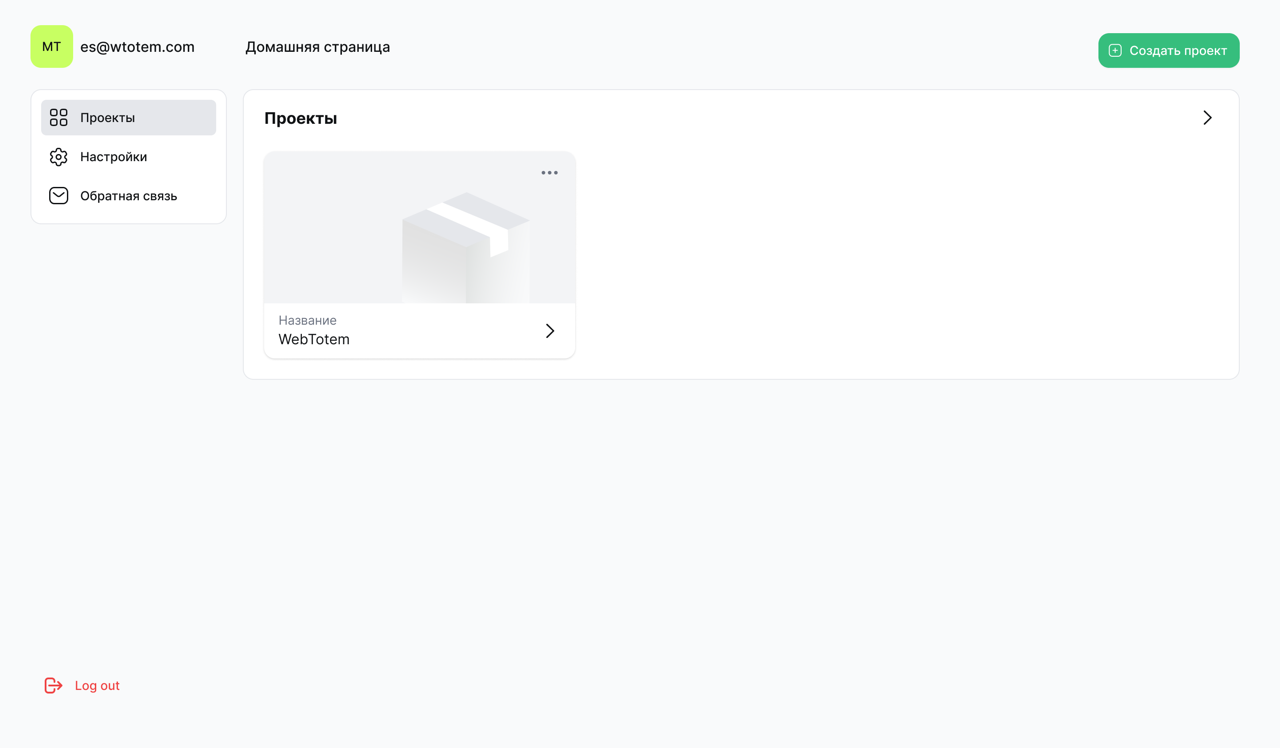
\includegraphics[width=0.6\textwidth]{media/ict/image19}
	\caption*{Рис. 2 - Панель управления}
\end{figure}

\begin{figure}[H]
	\centering
	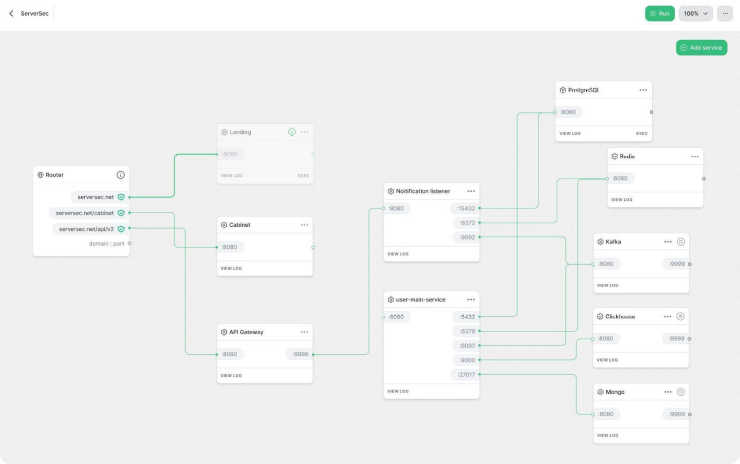
\includegraphics[width=0.6\textwidth]{media/ict/image20}
	\caption*{Рис. 3 - Запуск сервера}
\end{figure}

\begin{figure}[H]
	\centering
	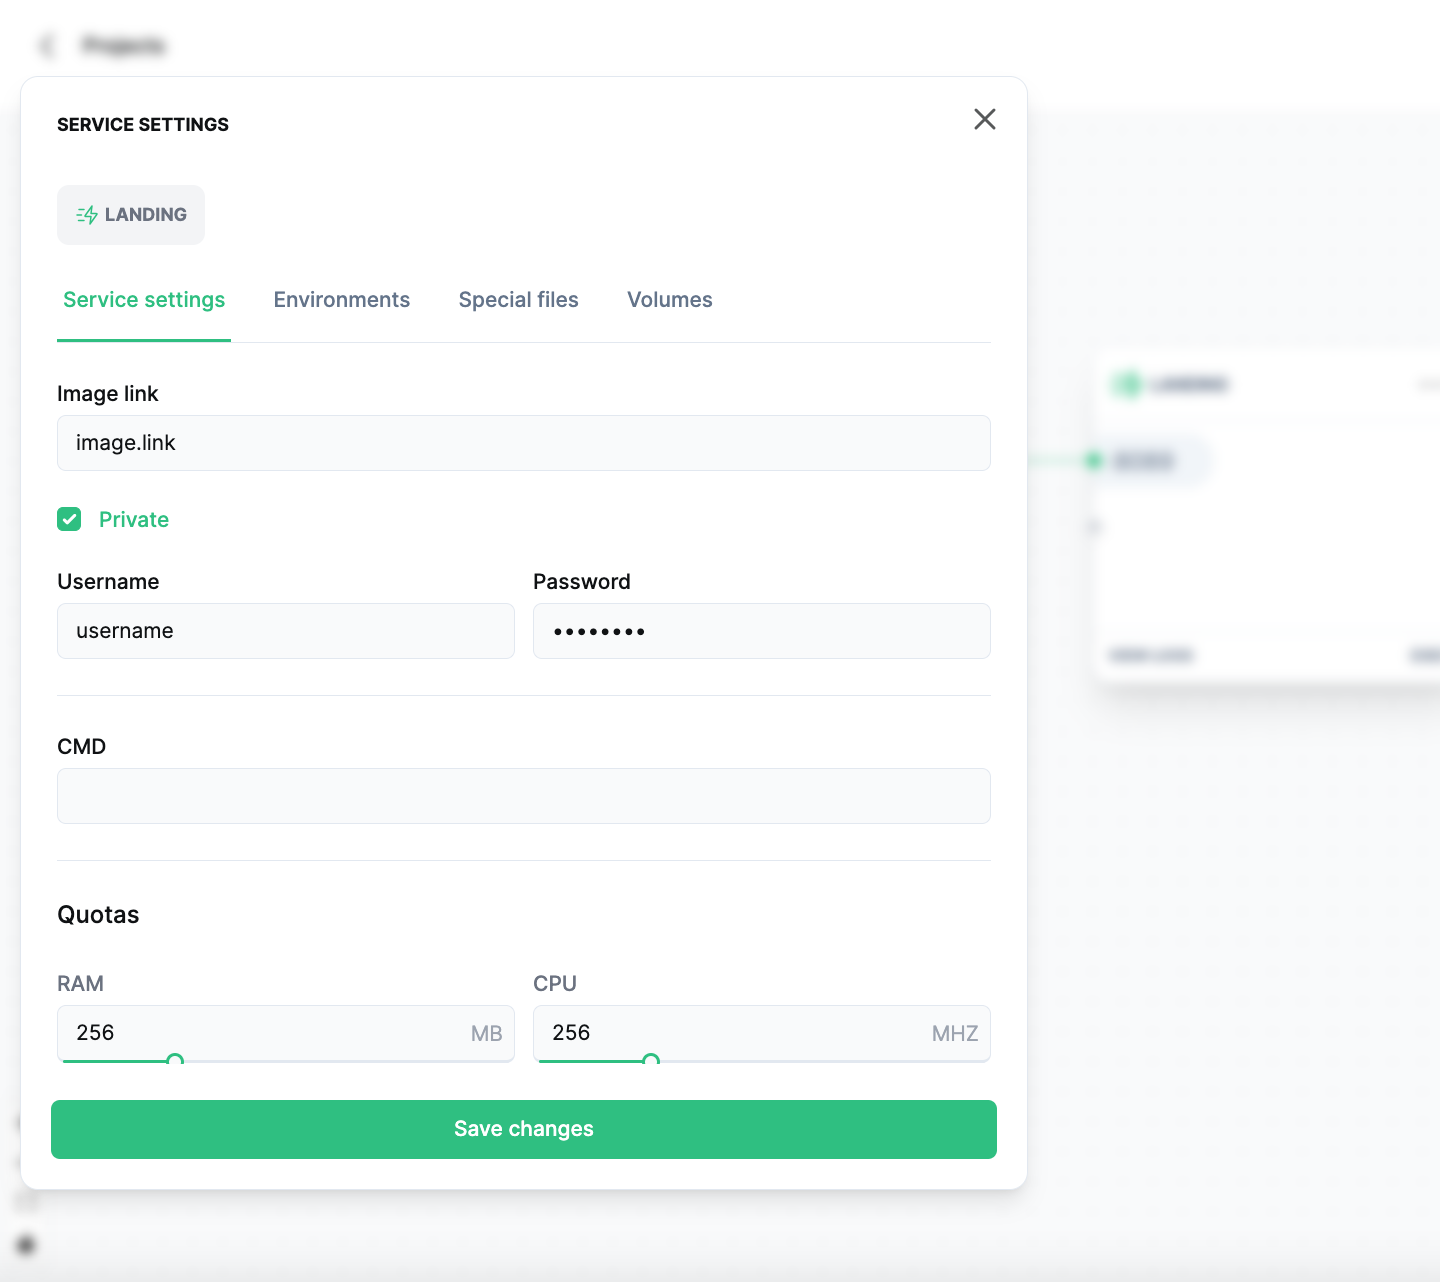
\includegraphics[width=0.6\textwidth]{media/ict/image21}
	\caption*{Рис. 4 - Пример параметров для запуска сервиса с использованием Docker}
\end{figure}

\begin{multicols}{2}
На платформе BULT процесс разработки и оркестрации веб-приложений
включает несколько ключевых этапов. Сначала проводится определение
требований и проектирование архитектуры, что включает сбор требований,
установление целей проекта и разработку структуры системы. Далее
разрабатываются микросервисы, которые упаковываются в контейнеры с
использованием технологий, таких как Docker, для обеспечения изоляции и
портативности. Затем осуществляется оркестрация контейнеров с помощью
инструментов, например, Nomad от HashiCorp, для управления ресурсами и
масштабируемости. После интеграции всех компонентов и их тестирования в
единой среде, система развертывается в продуктивной среде с
использованием инструментов автоматического развертывания и управления,
таких как Kubernetes и Terraform. Мониторинг и анализ работы приложений
осуществляются с помощью инструментов, таких как Grafana и Loki. На
завершающем этапе производится поддержка и обновление системы для
обеспечения безопасности и функциональности, а также внедрение новых
функций и исправление ошибок в рамках процесса DevOps.

Платформа BULT была разработана с учетом современных требований к
разработке и управлению веб-приложениями, обеспечивая высокий уровень
производительности и надежности. Она предлагает гибкость и
масштабируемость благодаря модульной архитектуре и поддержке
микросервисов, что позволяет легко адаптировать разработки к
изменяющимся требованиям. Удобный интерфейс личного кабинета упрощает
управление учетными данными и проектами, а поддержка Docker-образов и
файловых операций способствует эффективному управлению ресурсами.
Встроенные системы аутентификации и авторизации гарантируют защиту
данных и контроль доступа, в то время как многоязычная поддержка делает
платформу доступной для пользователей из разных регионов. Результаты
тестирования продемонстрировали снижение времени отклика системы на 26\%
и увеличение устойчивости под нагрузкой на 18\% по сравнению с
традиционными решениями, подтверждая конкурентоспособность платформы
BULT на рынке облачных технологий и ее способность удовлетворять
современные требования к управлению веб-приложениями.

Платформа BULT продемонстрировала значительное превосходство по
сравнению с традиционными подходами благодаря применению
междисциплинарного подхода, который интегрирует знания и методы из
информатики, инженерных наук, информационной безопасности и менеджмента.
Это позволило значительно повысить надежность и производительность
платформы, улучшив качество веб-приложений. Инновационные архитектурные
решения, такие как микросервисная архитектура и контейнеризация,
обеспечили высокую гибкость и масштабируемость, в то время как передовые
методы шифрования и защиты сетевого трафика повысили уровень
безопасности данных. Внедрение практик DevOps автоматизировало процессы
разработки, тестирования и развертывания, что сократило время на
внедрение новых функций и повысило стабильность системы. Таким образом,
междисциплинарный подход делает платформу BULT уникальным и эффективным
решением для современных задач облачных систем, предлагая высокую
производительность, надежность и гибкость.

{\bfseries Выводы.} В данной статье мы представили облачную платформу BULT,
которая использует передовые технологии для разработки и оркестрации
веб-приложений. Платформа BULT обеспечивает гибкость, масштабируемость и
надежность, предлагая решения для современных вызовов в области облачных
технологий. Более детальную информацию о платформе, её архитектурных
решениях и преимуществах можно найти на официальном сайте BULT {[}28{]}.
Этот ресурс предоставляет доступ к дополнительным материалам, примерам
применения и информации о технологических особенностях платформы, что
позволяет глубже понять её возможности и преимущества в сравнении с
традиционными подходами.

\emph{{\bfseries Финансирование.} Инициативный научный проект выполнен за
счет собственных средств ТОО «Web Totem» на основании протокола №1 от
10.11.23г. Регистрационный номер № 0124РКИ0205, Инвентарный №
0224РКИ0306.}
\end{multicols}

\begin{center}
{\bfseries Литература}
\end{center}

\begin{references}
1. Chen, L.~Microservices: Architecting for Continuous Delivery and
DevOps~// 2018 IEEE International Conference on Software Architecture
(ICSA). Seattle, WA, USA, 2018. - P. 39-397. DOI\\
10.1109/ICSA.2018.00013

2. Mazzara, M., Dragoni, N., Bucchiarone, A., Giaretta, A., Larsen, S.
T., Dustdar, S.~Microservices: Migration of a Mission Critical
System~// IEEE Transactions on Services Computing. - 2021. - Vol.
14(5)- P. 1464--1477. DOI 10.1109/TSC.2018.2889087

3. Singh, V., Peddoju, S. K.~Container-based Microservice Architecture
for Cloud Applications~// 2017 International Conference on Computing,
Communication and Automation (ICCCA). Greater Noida, India, 2017.- P.
847 - 852. DOI 10.1109/CCAA.2017.8229914

4. Villamizar, M., Garcés, O., Castro, H., Verano, M., Salamanca, L.,
Casallas, R., Gil, S.~Evaluating the Monolithic and the Microservice
Architecture Pattern to Deploy Web Applications in the Cloud~// 2015
10th Computing Colombian Conference (10CCC), 2015. -P. 583--590. DOI\\
10.1109/ColumbianCC.2015.7333476

5. Barinov, A., Morozov, I., Melnikov, K. V., Rudenko, E.~Agentless
Annotated Monitoring of User Behavioral Information in Container
Infrastructures~// Journal of the Ural Federal District. Information
Security. - 2023. -Vol. 23(1) DOI 10.14529/secur230102

6. Burns, B., Grant, B., Oppenheimer, D., Brewer, E., Wilkes, J.~Borg,
Omega, and Kubernetes: Lessons Learned from Three Container-Management
Systems over a Decade~// Queue. -2016. -Vol.14(1)- P. 70--93. DOI
10.1145/2898442.2898444

7. Baškarada, S., Nguyen, V., Koronios, A.~Architecting Microservices:
Practical Opportunities and\\ Challenges~// Journal of Computer
Information Systems. -2018. -Vol. 60(5) - P. 428--436. DOI\\
10.1080/08874417.2018.1520056

8. Balalaie, A., Heydarnoori, A., Jamshidi, P.~Microservices Architecture
Enables DevOps: Migration to a Cloud-Native Architecture~// IEEE
Software. -2016. -Vol. 33(3)- P. 42--52. DOI 10.1109/MS.2016.64

9. Omelchenko V., Rolik O. utomation of resource management in
information systems based on reactive vertical scaling// Адаптивні
Системи Автоматичного Управління. -2022. -Т.2(41)- С. 65 - 78. DOI
10.20535/1560-8956.41.2022.271344

10. Kusnandar, A.~Evaluation of Information System Security Using Fuzzy
FMEA Based on ISO/IEC 27001:2013 Framework to Improve Information
Security~//Journal of Business Information Systems. -2024.- Vol.14(2)-
P. 181- 190. DOI 10.21456/vol14iss2pp181-190

11. Cardarelli M., Iovino L., Francesco P. D., Salle A. D., Malavolta
I., Lago P. An extensible data-driven approach for evaluating the
quality of microservice architectures //~Proceedings of the 34th
ACM/SIGAPP Symposium on Applied Computing.- 2019.- P.1225-1234.

DOI
\href{https://doi.org/10.1145/3297280.3297400}{10.1145/3297280.3297400}

12. Femminella M., Palmucci M., Reali G., Rengo M. Attribute-based
management of secure Kubernetes cloud bursting //~IEEE Open Journal of
the Communications Society.-2024. -Vol. 5.- P. 1276 -1298. DOI
\href{https://doi.org/10.1109/ojcoms.2024.3367461}{10.1109/ojcoms.2024.3367461}

13. Desina G. C. Evaluating the impact of cloud-based microservices
architecture on application \\performance //arXiv preprint
arXiv:2305.15438. - 2023. DOI 10.48550/arXiv.2305.15438

14. Chen L., Xian M., \& Liu, J. Monitoring system of OpenStack cloud
platform based on Prometheus. 2020 International Conference on Computer
Vision, Image and Deep Learning (CVIDL). IEEE, pp. 206-209. DOI
10.1109/CVIDL51233.2020.0-100.

15. Wang M., Kulshrestha A., Wang L., Nordström L. Leveraging strategic
connection migration-powered traffic splitting for privacy
//~Proceedings on Privacy Enhancing Technologies.~-2022.-Vol.2022(3) -
P. 498 - 515.
DOI~\href{https://doi.org/10.56553/popets-2022-0083}{10.56553/popets-2022-0083}

16. Bezzateev S., Elina T. N., Mylnikov V. A. Modeling of selection
processes of cloud systems parameters providing their stability in
accordance with reliability and safety //~Scientific and Technical
Journal of Information Technologies, Mechanics and Optics.- 2018.-Vol.
18(4) - P. 654- 662. DOI
\href{https://doi.org/10.17586/2226-1494-2018-18-4-654-662}{10.17586/2226-1494-2018-18-4-654-662}

17. Hung M.-H., Lin Y.-C., Hsiao H.-C., Chen C.-C., Lai K.-C., Hsieh
Y.-M., Tieng H., Tsai T.-H., Huang H.-C., Yang H.-C., Cheng F.-T. A
novel implementation framework of digital twins for intelligent
manufacturing based on container technology and cloud manufacturing
services // IEEE Transactions on Automation Science and Engineering.-
2022.-Vol.19(3)- P.1614- 1630. DOI10.1109/TASE.2022.3143832

18. Kale S., et al. E-FireGuard: Empowering firefighters through
innovative E-commerce solutions \\//~Industrial Management
Advances. -2024.-Vol.2(1)- P. 6375--6375.
DOI 10.59429/ima.v2i1.6375

19. Тарамов А.А., Черненькая Л.В. Описание инструментария для создания
современного CI/CD конвейера //Перспективы науки. -- 2020. - №12(135).-
С.74-77.

20. Безпятый М. В. Автоматизация и оптимизация процессов разработки и
развертывания в devops: применение современных методов и инструментов
//Инновации и инвестиции. -- 2023.- №. 7. - С. 458-464.

21. Брыжинская А.В., Чернова С.В. КРАТКО ПРО DOCKER // Теория и практика
современной науки. 2019. -№10 (52). - С. 33-35.

22. Munisso R., Chis A. E. Cloudmapper: A model-based framework for
portability of cloud applications consuming PaaS services//2017 25th
Euromicro International Conference on Parallel, Distributed and
Network-Based Processing (PDP).-2017.- P.132-139. DOI
10.1109/pdp.2017.94

23. PostgreSQL Documentation. URL:
\url{https://www.postgresql.org/docs/-}Дата обращения: 28.08.2024.

24. Lee J.,Kim M.,Shah S.A.R., Ahn S.U.,Yoon H.,Noh S.Y.Performance
evaluations of distributed file systems for scientific big data in FUSE
environment//Electronics.-2021.-Vol.10 (12) - P. 1471. DOI \\
\href{https://doi.org/10.3390/electronics10121471}{10.3390/electronics10121471}

25. Grafana Documentation. URL: \url{https://grafana.com/docs/-} Дата
обращения: 28.08.2024.

26. Loki Documentation. URL: \url{https://grafana.com/oss/loki/} - Дата
обращения: \\28.08.2024.

27. Тюменцев Д. В. Devops в эпоху облачных технологий: современные
практики и перспективы развития //Вестник науки.- 2023.-Т.2. -№. 8
(65).- С. 190-195.

28. BULT. {[}Электронный ресурс{]}. URL: \url{https://bult.pro-} Дата
обращения: 28.08.2024
\end{references}

\begin{center}
{\bfseries References}
\end{center}

\begin{references}
1. Chen, L.~Microservices: Architecting for Continuous Delivery and
DevOps~// 2018 IEEE International Conference on Software Architecture
(ICSA). Seattle, WA, USA, 2018. - P. 39-397.

DOI 10.1109/ICSA.2018.00013

2. Mazzara, M., Dragoni, N., Bucchiarone, A., Giaretta, A., Larsen, S.
T., Dustdar, S.~Microservices: Migration of a Mission Critical System~//
IEEE Transactions on Services Computing. - 2021. - Vol. 14(5)- P.
1464--1477. DOI 10.1109/TSC.2018.2889087

3. Singh, V., Peddoju, S. K.~Container-based Microservice Architecture
for Cloud Applications~// 2017 International Conference on Computing,
Communication and Automation (ICCCA). Greater Noida, India, 2017.- P.
847 - 852. DOI 10.1109/CCAA.2017.8229914

4.Villamizar, M., Garcés, O., Castro, H., Verano, M., Salamanca, L.,
Casallas, R., Gil, S.~Evaluating the Monolithic and the Microservice
Architecture Pattern to Deploy Web Applications in the Cloud~// 2015
10th Computing Colombian Conference (10CCC), 2015. -P. 583--590. DOI
\\10.1109/ColumbianCC.2015.7333476

5. Barinov, A., Morozov, I., Melnikov, K. V., Rudenko, E.~Agentless
Annotated Monitoring of User Behavioral Information in Container
Infrastructures~// Journal of the Ural Federal District. Information
Security. - 2023. -Vol. 23(1) DOI 10.14529/secur230102

6. Burns, B., Grant, B., Oppenheimer, D., Brewer, E., Wilkes, J.~Borg,
Omega, and Kubernetes: Lessons Learned from Three Container-Management
Systems over a Decade~// Queue. -2016. -Vol.14(1)- P. 70--93. DOI
10.1145/2898442.2898444

7. Baškarada, S., Nguyen, V., Koronios, A.~Architecting Microservices:
Practical Opportunities and \\Challenges // Journal of Computer
Information Systems. -2018. -Vol. 60(5) - P. 428--436. DOI \\
10.1080/08874417.2018.1520056

8. Balalaie, A., Heydarnoori, A., Jamshidi, P.~Microservices Architecture
Enables DevOps: Migration to a Cloud-Native Architecture~// IEEE
Software. -2016. -Vol. 33(3)- P. 42--52. DOI 10.1109/MS.2016.64

9. Omelchenko V., Rolik O. utomation of resource management in
information systems based on reactive vertical scaling// Адаптивні
Системи Автоматичного Управління. -2022. -Т.2(41)- С. 65 - 78. DOI
10.20535/1560-8956.41.2022.271344

10. Kusnandar, A.~Evaluation of Information System Security Using Fuzzy
FMEA Based on ISO/IEC 27001:2013 Framework to Improve Information
Security~//Journal of Business Information Systems. -2024.- Vol.14(2)-
P. 181- 190. DOI 10.21456/vol14iss2pp181-190

11. Cardarelli M., Iovino L., Francesco P. D., Salle A. D., Malavolta
I., Lago P. An extensible data-driven approach for evaluating the
quality of microservice architectures //~Proceedings of the 34th
ACM/SIGAPP Symposium on Applied Computing.- 2019.- P.1225-1234.

DOI
\href{https://doi.org/10.1145/3297280.3297400}{10.1145/3297280.3297400}

12. Femminella M., Palmucci M., Reali G., Rengo M. Attribute-based
management of secure Kubernetes cloud bursting //~IEEE Open Journal of
the Communications Society.-2024. -Vol. 5.- P. 1276 -1298. DOI
\href{https://doi.org/10.1109/ojcoms.2024.3367461}{10.1109/ojcoms.2024.3367461}

13. Desina G. C. Evaluating the impact of cloud-based microservices
architecture on application \\performance //arXiv preprint
arXiv:2305.15438. - 2023. DOI 10.48550/arXiv.2305.15438

14. Chen L., Xian M., \& Liu, J. Monitoring system of OpenStack cloud
platform based on Prometheus. 2020 International Conference on Computer
Vision, Image and Deep Learning (CVIDL). IEEE, pp. 206-209. DOI
10.1109/CVIDL51233.2020.0-100.

15. Wang M., Kulshrestha A., Wang L., Nordström L. Leveraging strategic
connection migration-powered traffic splitting for privacy
//~Proceedings on Privacy Enhancing Technologies.~-2022.-Vol.2022(3) -
P. 498 - 515.
DOI~\href{https://doi.org/10.56553/popets-2022-0083}{10.56553/popets-2022-0083}

16. Bezzateev S., Elina T. N., Mylnikov V. A. Modeling of selection
processes of cloud systems parameters providing their stability in
accordance with reliability and safety //~Scientific and Technical
Journal of Information Technologies, Mechanics and Optics.- 2018.-Vol.
18(4) - P. 654- 662. DOI
\href{https://doi.org/10.17586/2226-1494-2018-18-4-654-662}{10.17586/2226-1494-2018-18-4-654-662}

17. Hung M.-H., Lin Y.-C., Hsiao H.-C., Chen C.-C., Lai K.-C., Hsieh
Y.-M., Tieng H., Tsai T.-H., Huang H.-C., Yang H.-C., Cheng F.-T. A
novel implementation framework of digital twins for intelligent
manufacturing based on container technology and cloud manufacturing
services // IEEE Transactions on Automation Science and Engineering.-
2022.-Vol.19(3)- P.1614- 1630. DOI10.1109/TASE.2022.3143832

18. Kale S., et al. E-FireGuard: Empowering firefighters through
innovative E-commerce solutions \\//~Industrial Management
Advances. -2024.-Vol.2(1)- P. 6375--6375. DOI 10.59429/ima.v2i1.6375

19. Taramov A.A., Chernen' kaja L.V. Opisanie
instrumentarija dlja sozdanija sovremennogo CI/CD \\konvejera
//Perspektivy nauki. -- 2020. - №12(135).- S.74-77.{[}in Russian{]}

20. Bezpjatyj M. V. Avtomatizacija i optimizacija processov razrabotki i
razvertyvanija v devops: \\primenenie sovremennyh metodov i instrumentov
//Innovacii i investicii. -- 2023.- №. 7. - S. 458-464.

21.Bryzhinskaja A.V., Chernova S.V. KRATKO PRO DOCKER // Teorija i
praktika sovremennoj

nauki. 2019. -№10 (52). - S. 33-35. {[}in Russian{]}

22. Munisso R., Chis A. E. Cloudmapper: A model-based framework for
portability of cloud applications consuming PaaS services//2017 25th
Euromicro International Conference on Parallel, Distributed and
Network-Based Processing (PDP).-2017.- P.132-139. DOI
10.1109/pdp.2017.94

23. PostgreSQL Documentation. URL:
\url{https://www.postgresql.org/docs/-}Дата обращения: 28.08.2024.

24.Lee J.,Kim M.,Shah S.A.R., Ahn S.U.,Yoon H.,Noh S.Y.Performance
evaluations of distributed file systems for scientific big data in FUSE
environment//Electronics.-2021.-Vol.10 (12) - P. 1471. DOI\\
\href{https://doi.org/10.3390/electronics10121471}{10.3390/electronics10121471}

25. Grafana Documentation. URL: \url{https://grafana.com/docs/-} Data
obrashhenija: 28.08.2024.

26. Loki Documentation. URL: \url{https://grafana.com/oss/loki/} - Data
obrashhenija: \\28.08.2024.

27. Tjumencev D. V. Devops v jepohu oblachnyh tehnologij: sovremennye
praktiki i perspektivy razvitija //Vestnik nauki.- 2023.-T.2. -№. 8
(65).- S. 190-195.{[}in Russian{]}

28. BULT. {[}Электронный ресурс{]}. URL: \url{https://bult.pro-} Data
obrashhenija: 28.08.2024.
\end{references}

\begin{authorinfo}
\emph{{\bfseries Сведения об авторах}}

Шайханова А.К.- PhD, и.о. профессора кафедры информационной
безопасности, Евразийский национальный университет имени Л.Н.Гумилева,
Астана, Казахстан, e-mail:
\href{mailto:shaikhanova_ak@enu.kz}{\nolinkurl{shaikhanova\_ak@enu.kz}};

Бермухамбетов Ж.А.-Технический директор ТОО «WebTotem», e-mail:
\href{mailto:zb@wtotem.com}{\nolinkurl{zb@wtotem.com}};

Ким В.В.- Главный архитектор ТОО «WebTotem», Астана, Казахстан, e-mail:
\href{mailto:vk@wtotem.com}{\nolinkurl{vk@wtotem.com}};

Тлеубаева А.О.- докторант ТОО «Astana IT University», Астана, Казахстан,
e-mail:
\href{mailto:Arailym.tll@gmail.com}{\nolinkurl{Arailym.tll@gmail.com}}

\emph{{\bfseries Information about the authors}}

Shaikhanova A. K.-PhD, Acting Professor, Department of Information
Security, L.N. Gumilyov Eurasian National University, Astana,
Kazakhstan, e-mail:
\href{mailto:shaikhanova_ak@enu.kz}{\nolinkurl{shaikhanova\_ak@enu.kz}};

Bermukhambetov Zh.A.- Technical Director of LLP "WebTotem", Astana,
Kazakhstan, e-mail:
\href{mailto:zb@wtotem.com}{\nolinkurl{zb@wtotem.com}};

Kim V.V.- Chief Architect of LLP "WebTotem, Astana, Kazakhstan,
e-mail:\href{mailto:vk@wtotem.com}{\nolinkurl{vk@wtotem.com}};

Tleubayeva A.O. - PhD student of LLP «Astana IT University», Astana,
Kazakhstan, e-mail: Arailym.tll@gmail.com
\end{authorinfo}
